\documentclass{article}
\usepackage{graphicx} % Required for inserting images
\usepackage[utf8]{inputenc}
\usepackage[T1]{fontenc}
\usepackage{karnaugh-map}
\usepackage[polish]{babel}
\usepackage{subcaption}
\usepackage{float}
\usepackage{enumitem}
\usepackage{url}
\usepackage{array}
\usepackage{indentfirst}


\begin{document}

\begin{center}
	% Używamy @{} aby usunąć zewnętrzne marginesy
	% Używamy 'm' (z pakietu 'array') dla środkowania w pionie
	
	\begin{tabular}{@{}|m{0.65\textwidth}|m{0.3\textwidth}|@{}}
		\hline
		% --- PIERWSZY WIERSZ LOGICZNY (wg obrazka) ---
		% Komórka 1,1 (Lewa-góra)
		Wydział Informatyki Politechniki Białostockiej \newline
		Przedmiot: Modułowe systemy cyfrowe
		&
		% Komórka 1,2 (Prawa-góra)
		Data: 28.10.2025 \\ \hline
		
		% --- DRUGI WIERSZ LOGICZNY (wg obrazka) ---
		% Komórka 2,1 (Lewa-środek)
		Zajęcia nr 2 \newline
		Temat: Bloki kombinacyjne: multipleksery, demultipleksery i dekodery \newline
		
		& % <-- Separator kolumn dla wiersza 2
		
		% Komórka 2,2 (Prawa-środek)
		
		\\
		
		% --- TRZECI WIERSZ LOGICZNY (wg obrazka) ---
		% Komórka 3,1 (Lewa-dół)
		Grupa: Lab 8 \newline
		Imię i nazwisko: \newline
		Kamil Kubajewski, Jakub Matusiewicz, Bartosz Orłowski
		
		& % <-- Separator kolumn dla wiersza 3
		
		% Komórka 3,2 (Prawa-dół)
		Prowadzący: \newline
		dr hab. inż. Sławomir Zieliński \\ \hline
	\end{tabular}
\end{center}

\section{Cel ćwiczeń}

Zapoznanie z podstawowymi kombinacyjnymi układami scalonymi, konkretnie \textbf{multiplekserami}, \textbf{demultiplekserami} i \textbf{dekoderami}.

\section{Podstawa teoretyczna}

Na zajęciach będziemy zajmować się kombinacyjnymi
układami scalonymi. Stan wyjść w tych układach zależy wyłącznie od
aktualnego stanu wejść, a stan wyjść są opisywane za pomocą funkcji boolowskich\cite{maciak,wiki}.\\

Do bloków kombinacyjnych zalicza się:
\begin{itemize}
	\item Komulatory - multiplekser, demultiplekser
	\item Konwertery kodów - koder, dekoder, transkoder
	\item Bloki arytmetyczne - sumator, komparator, ALU
\end{itemize}

W układach cyfrowych może wystąpić zjawisko hazardu, którego podłożem jest niezerowy czas propagacji sygnałów. Oznacza to, że sygnały podane na wejście biegną do wyjścia różnymi ścieżkami logicznymi, z których każda może mieć inny sumaryczny czas opóźnienia. Zanim układ osiągnie swój nowy, stabilny stan, ta różnica w czasie dotarcia sygnałów może spowodować pojawienie się na wyjściu krótkotrwałego, niepożądanego impulsu\cite{wiki}.\\

\pagebreak

Multiplekser
(MUX)-  Działa jak selektor danych.
Posiada $2^n$ wejść danych, $n$ wejść sterujących i jedno wyjście. Zadaniem
multipleksera jest przełączenie sygnału z jednego wybranego wejścia danych $D_i$
na wyjście $Y$. Wybór aktywnego wejścia jest dokonywany za pomocą kodu
binarnego podanego na wejścia sterujące\cite{maciak}.
\begin{figure}[h]
	\centering
	\includegraphics[width=0.50\textwidth]{Obwod1_1.PNG}
	\caption{Schemat 2-wejściowego multipleskera}
	\label{fig:moj_obrazek}
\end{figure}

Demultiplekser
     (DEMUX)- Działa odwrotnie do multipleksera, czyli  rozdziela dane. Posiada jedno wejście
     danych, $n$ wejść sterujących i $2^n$ wyjść. Demultiplekser przesyła
     sygnał z wejścia danych $D$ na jedno wybrane wyjście $Y_i$. Wybór
     aktywnego wyjścia jest dokonywany przez kod binarny na wejściach sterujących
     . Pozostałe wyjścia przyjmują nieaktywny stan logiczny, czyli ,,0''\cite{maciak}.
\begin{figure}[h]
	\centering
	\includegraphics[width=0.50\textwidth]{Obwod2.PNG}
	\caption{Schemat 4-wyjściowego demultipleksera}
	\label{fig:moj_obrazek}
\end{figure}

Dekoder-
     Konwertuje $n$-bitowy kod wejściowy na sygnał wyjściowy, pojawiający
     się na jednym z $m$ wyjść (gdzie $m \le 2^n$). 
Jednym z dekoderów jest dekoder ,,1
z n''. Dla każdej unikalnej kombinacji binarnej na wejściach, aktywowane jest jedno,
odpowiadające jej wyjście. Pozostałe wyjścia pozostają w stanie nieaktywnym.
Innym dekoderem jest Dekoder
BCD na 7-segmentowy. Służy on do sterowania wyświetlaczem 7-segmentowym.Otrzymuje 4-bitowy kod BCD, który reprezentuje cyfry dziesiętne od 0
do 9. Posiada on 7 wyjść oznaczanych od 'a' do 'g', z których każde
odpowiada jednemu segmentowi na wyświetlaczu. Układ zawiera wewnętrzną
logikę, która dla danego kodu BCD na wejściu aktywuje odpowiednią kombinację
wyjść (segmentów), aby na wyświetlaczu pojawiła się właściwa cyfra\cite{maciak}.
\begin{figure}[h]
	\centering
	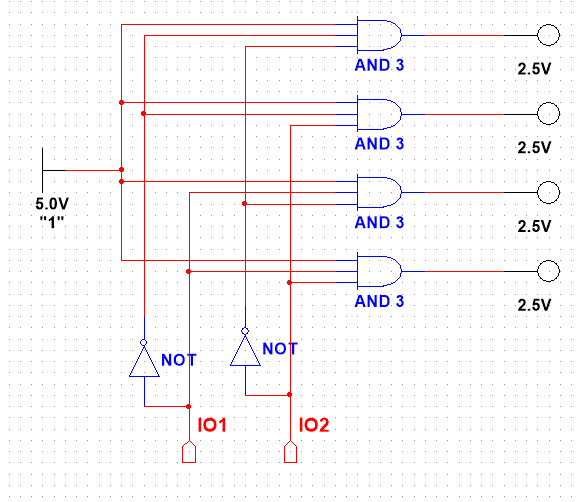
\includegraphics[width=0.50\textwidth]{dekoder.PNG}
	\caption{Schemat 4-wyjściowego dekodera}
	\label{fig:moj_obrazek}
\end{figure}\\

    \pagebreak

\pagebreak
\section{Przebieg ćwiczeń}
\subsection{Zadanie 1}
Zrealizować multiplekser dwuwejściowy na bramkach logicznych (DB10).
\begin{figure}[h]
    \centering
    \includegraphics[width=0.50\textwidth]{Obwod1_1.PNG}
    \caption{Obwód do zadania 1 i 2}
    \label{fig:moj_obrazek}
\end{figure}\\

Multiplekser dwuwejściowy posiada dwa wejścia danych oraz jedną linię sterującą. Jego budowa opiera się na dwóch bramkach \textbf{AND}, których wyjścia podłączone są do wejść dwuwejściowej bramki \textbf{OR}, co pozwala na wybór aktywnego wejścia. Do przetestowania układu użyto modułu \textbf{DB10}, wykorzystując przełączniki do zadawania stanów logicznych \textbf{0} lub \textbf{1} na wejściach i linii sterującej.

\subsection{Zadanie 2}
Zrealizować multiplekser czterowejściowy na bramkach logicznych (DB10).
\begin{figure}[h]
    \centering
    \includegraphics[width=0.50\textwidth]{Obwod1.PNG}
    \caption{Obwód do zadania 1 i 2}
    \label{fig:moj_obrazek}
\end{figure}\\
Multiplekser czterowejściowy posiada cztery wejścia danych oraz dwie linie sterujące. Jego budowa opiera się na czterech bramkach \textbf{AND}, których wyjścia podłączone są do wejść czterowejściowej bramki \textbf{OR}, co pozwala na wybór aktywnego wejścia. Do przetestowania układu użyto modułu \textbf{DB10}, wykorzystując przełączniki do zadawania stanów logicznych \textbf{0} lub \textbf{1} na wejściach i liniach sterujących.

\pagebreak
\subsection{Zadanie 3}
Zrealizować demultiplekser na bramkach logicznych (DB10)
\begin{figure}[h]
    \centering
    \includegraphics[width=0.50\textwidth]{Obwod2.PNG}
    \caption{Obwód do zadania 3}
    \label{fig:moj_obrazek}
\end{figure}\\
Demultiplekser jednowejściowy z czterema wyjściami składa się z jednego wejścia danych i dwóch linii sterujących. Podłączając bramkę NOT do wejść linii sterujących i cztery bramki AND, możemy kierować sygnał z wejścia na wybrane wyjście. Do przetestowania użyto modułu \textbf{DB10}, do którego podłączono przełączniki dla zmiany sygnałów 0 lub 1.
\pagebreak
\subsection{Zadanie 4}
Przebadać blok funkcjonalny z dekoderem DB31. Zrealizować dekodery kodu 1 z 8 oraz 1 z 16.
\begin{figure}[h]
    \centering
    \includegraphics[width=0.50\textwidth]{Obwod2.PNG}
    \caption{Obwód do zadania 3}
    \label{fig:moj_obrazek}
\end{figure}\\

Do przetestowania sygnałów od 1 z 8 oraz 1 z 16 wykorzystano moduł DB31 poprzez podłączenie zegaru taktującego do wejścia CLK, do wejść G1 oraz $\overline{G2B}$ podłączono przełączniki do wysyłania stałej jedynki, a wyjścia od Y14 do Y17 oraz od Y20 do Y23 podłączono do diód wyjściowych, które wyświetlały 4 najmłodsze bity z pierwszej ósemki i 4 najmłodsze bity z drugiej ósemki. Za pomocą takiego połączenia osiągnięto sygnał na wyjściu odpowiadający danym liczbom.
\pagebreak
\subsection{Zadanie 5}
Zrealizować dekoder kodu BCD z wyjściem na wyświetlacz 7 – segmentowy (DB15).
\begin{figure}[h]
    \centering
    \includegraphics[width=0.50\textwidth]{Obwod3.PNG}
    \caption{Obwód do zadania 5}
    \label{fig:moj_obrazek}
\end{figure}\\
Do przetestowania dekodera BCD na 7-segmentowy wyświetlacz użyto modułu \textbf{DB15}. Moduł ten zawiera układ scalony \textbf{74LS47} oraz zintegrowany \textbf{wyświetlacz 7-segmentowy}. Za pomocą przełączników podawano na wejścia $A_0$-$A_3$ układu 4-bitowe kombinacje kodu BCD, odpowiadające cyfrom od 0 do 9. Sprawdzono, że dla każdej podanej kombinacji na wyświetlaczu pojawiała się poprawna cyfra.

\pagebreak
\section{Dyskusja błedów}
%Klasyczna formułka np. z EDI, jaka powinna byc oczekiwana wartość? Bład ludzki, niedokładnosc przyrządów, itd

W przeprowadzonych zadaniach badano działanie układów kombinacyjnych cyfrowych. Pomiary te miały charakter czysto funkcjonalny, czyli sprwadzenie czy dany układ działa według założeń teoretycznych. Podczas obserwacji nie zaobserwowano istotnych błędów w działaniu układów kombinacyjnych. Wszystkie układy, czyli multipleksery, demultipleksery oraz dekodery działały zgodnie z teorią oraz z tabelami prawdy. Wyniki praktyczne odpowiiadały wartościom oczekiwanym, a wskazania stanów logicznych na wyjściach były zgodne z przewidywaniami dla poszczególnych kombinacji sygnałów wejściowych.\\

W trackie wykonywania zadań mogły wystąpić chwilowe zjawiska przejściowe wynikające z właściwości fizycznych układów, takich jak hazard lub wyścig, które mogą powodować krótkotrawłe zmiany sygnałów na wyjściu przy przełączaniu wejść. Zjawiska te są typowe dla układów opartych na bramkach logicznych i nie wpływają znacząco na poprawne działanie układu.\\

W zadaniu pierwszy oraz drugim badano działanie multiplekserów 2- i 4-wejściowego. Podawane stany logiczne 0 lub 1 na wejściach oraz liniach sterujących pozwoliły na potwierdzenie poprawności działania multiplekserów zgodne z teorią. Teoretycznie mogłyby wystąpić krótkotrwałe przejściowe zmiany stanów tzw. hazard statyczny, jednak nie były one zauważalne i nie miały wpływu na wyniki.\\

W zadaniu trzecim demultiplekser poprawnie kierował sygnał z jednego wejścia na odpowiednie wyjście podając na wejścia dancyh oraz linie sterujące odpowiednie stany logiczne. Nie odnotowano błędnych stanów, choć przy przełączaniu wejść mogły pojawić się chwilowe przejściowe stany na więcej niż jednym wyjściu (typowy efekt propagacji sygnału).\\

W zadaniu czwartym działanie dekodera było zgodne z oczekiwaniami. Układ na platformie do testowania Scientech 2611 podłączono w taki sposób, aby na ośmiu diodach LED wyświetlać kolejno cztery najmłodsze bity (1–4), a następnie cztery starsze (9–12). W efekcie diody świeciły w sekwencji:
0(1), 1(1), 2(1), 3(1), 4(0), 5(0), 6(0), 7(0),
a następnie w odwrotnej kolejności. Dekoder był sterowany sygnałem zegarowym, dzięki czemu kolejne diody zapalały się po sobie w rytmie taktowania, odwzorowując pracę licznika binarnego. Układ działał stabilnie i zgodnie z oczekiwaniami, nie wykazując błędów w przełączaniu stanów. Wahania w czasie przejść mogły wynikać jedynie z charakterystycznych dla bramek logicznych opóźnień propagacji.\\
W zadaniu piątym dekoder BCD działał prawidłowo i tłumaczył podane kombinacje kodu za pomocą przełączników  podłączonych od wejść $A_0$ do $A_3$, a wynik wyświetlano na wyświetlaczu siedmiosegmentowym. Układ działał zgodnie z teorią i nie zaobserwowano żadnych błędów. 

\pagebreak
\section{Wnioski}
Na zajęciach zapoznaliśmy się z budową i zasadą działania układów
kombinacyjnych: multiplekser, demultiplekser i dekoder. Realizacja
multiplekserów potwierdziły, że multiplekser działa jak sterowany
cyfrowo przełącznik. Zaobserwowaliśmy, że liczba $n$ linii sterujących
determinuje liczbę $2^n$ wejść danych, z których można dokonać selekcji. Demultiplekser
działał odwrotnie. Układ kierował sygnał z jednego wejścia danych na jedno z $2^n$
wyjść, zgodnie z kodem binarnym podanym na $n$ wejść sterujących. Pozostałe
wyjścia pozostawały w stanie niskim. Dekoder "1 z n" ustawiał
stan '1' lub '0' w zależności od typu wyjść. Wyjście zależało od liczby
binarnej podanej na wejście. Dekoder BCD na 7-segmentowy wyświetlacz poprawnie
tłumaczył 4-bitowy kod BCD na odpowiednią kombinację 7 sygnałów wyjściowych
(segmentów od 'a' do 'g') oraz wyświetlał właściwe cyfry dziesiętne.

\section{Literatura}

\renewcommand{\refname}{}

\begin{thebibliography}{9}
    
    \bibitem{maciak} 
    T. Maciak, \textit{Skrypt do laboratorium Elektroniki cyfrowe}, 
    Wydział Informatyki Politechniki Białostockiej, Białystok, 2021.
    
    \bibitem{wiki} 
    \textit{Układ Kombinacyjny}, Wikipedia, dostęp online: 
    \url{https://pl.wikipedia.org/wiki/Uk%C5%82ad_kombinacyjny}, 
    data dostępu: luty 2023.
    
    
\end{thebibliography}

\pagebreak
\section{Protokół}

\begin{figure}[h]
    \centering
    \includegraphics[width=1\textwidth, angle=-90]{protokol.JPG}
    \caption{Protokół}
    \label{fig:moj_obrazek}
\end{figure}
\end{document}
